\documentclass{article}
\usepackage[english]{babel}
\usepackage{amsmath,amssymb,graphicx,hyperref}

%%%%%%%%%% Start TeXmacs macros
\catcode`\>=\active \def>{
\fontencoding{T1}\selectfont\symbol{62}\fontencoding{\encodingdefault}}
\newcommand{\tmem}[1]{{\em #1\/}}
\newcommand{\tmtextbf}[1]{{\bfseries{#1}}}
%%%%%%%%%% End TeXmacs macros

\newcommand{\maxwidth}{{\ifdim}{\Ginnatwidth}>tex-line-widthtex-line-width{\else}{\Ginnatwidth}{\tmfi}}
\newcommand{\maxheight}{{\ifdim}{\Ginnatheight}>tex-text-heighttex-text-height{\else}{\Ginnatheight}{\tmfi}}
\newcommand{\tightlist}{}
\newcommand{\fps}{htbp}

\begin{document}

\date{}

\maketitle

\section*{2. Probability Distribution}\label{header-n0}

{\tmem{Density estimation}}

$\quad \quad$Data points are independent and identically distributed. There
are infinitely many probability distributions that could have given rise to
the observed finite data set.

\tmtextbf{Parametric} and \tmtextbf{non-parametric} approaches.

\section*{3. Linear Models for Regression}\label{header-n10}

$\quad \quad$The goal of regression is to predict the value of one or more
continuous {\tmem{target}} variables $t$ given the value of a $D$-dimensional
vector $\vec{x}$ {\tmem{input}} variables.

\subsection*{3.1 Linear Basis Function Models}\label{header-n13}

\begin{align}
  y (x, w) = & w_0 + \sum^{M - 1}_{j = 1} w_j \phi_j (x)\\
  = & w^T \phi (x)
\end{align}

where $\phi_j (\vec{x})$ are known as {\tmem{basis functions}}, and $w_0$
{\tmem{bias}} parameter.\\
$w = (w_0, ..., w_{M - 1})^T$ and $\phi = (\phi_0, ..., \phi_{M - 1})^T$.

$\quad \quad$By using nonlinear basis functions, we allow the function $y (x,
w)$ to be a non-linear function of the input vector $x$. Thus Eq. above is
called a {\tmem{linear model}}.

\tmtextbf{Choices for the basis functions}

{\tmem{Gaussian}}:
\[ \phi_j (x) = exp \left\{ - \frac{(x - \mu_j)^2}{2 s^2} \right\} \]
where $\mu_j$ govern the locations of the basis functions in input space.

{\tmem{Sigmoidal basis function}}:

\begin{align}
  & \quad \quad \quad \phi_j (x) = \sigma (\frac{x - \mu_j}{s})\\
  & \text{where: }\\
  & \quad \qquad \sigma (a) = \frac{1}{1 + exp (- a)}
\end{align}

and $tanh (a) = 2 \sigma (a) - 1$

{\tmem{the Fourier basis}}: Each basis function represents a specific
frequency and has infinite spatial extent.

\paragraph{Maximum Likelihood and least squares}\label{header-n34}

\href{https://en.wikipedia.org/wiki/Mode_(statistics)}{Mode}

$\quad \quad$Assume $p (t, |X, w, \beta) = \mathcal{N} (t|y, \beta^{- 1})$,
where $t = y + \epsilon$ and $y = w^T \phi (x)$

\begin{align}
  p (\mathrm{t} |X, w, \beta) & = \prod^N_{n = 1} \mathcal{N} (t_n |w^T \phi
  (x_n), \beta^{- 1})\\
  & = \frac{N}{2} ln \beta - \frac{N}{2} ln (2 \pi) - \beta E_D (w)\\
  & 
\end{align}

where $\mathrm{t}$ is the column vector of targets and $E_D (w) = \frac{1}{2}
\sum^N_{n = 1} \{t_n - w^T \phi (x_n)\}^2$. It is easy to see that
maximization of the likelihood function under a conditional Gaussian noise
distribution for a linear model is equivalent to minimizing a sum-of-squares
error function. Take the gradient and set it to zero:
\[ w_{ML} = (\Phi^T \Phi)^{- 1} \Phi^T \mathrm{t} \]
where {\tmem{design matrix}} $\Phi$ is given by $\Phi_{nj} = \phi_j (x_n)$

$\quad \quad$Take the derivative w.r.t. $w_0$
\[ w_0 = \bar{t} - \sum^N_{j = 1} w_j  \bar{\phi}_j \]
where $\bar{t}$ and $\overline{\phi_j}$ are the arithmetic mean of their
elements.

$\quad \quad$Maximize the log likehood w.r.t. the noise precision parameter
$\beta$:
\[ \frac{1}{\beta_{ML}} = \frac{1}{N} \sum^N_{n = 1} [t_n - w^T_{ML} \phi
   (x_n)]^2 \]
$\quad \quad$The least-squares regression function (Euclidean distance) is
obtained by finding the orthogonal projection of the data vector $t$ onto the
subspace spanned by the basis functions $\phi_j (x)$ in which each basis
function is viewed as a vector $\phi_j$ of length {\tmem{N}} with elements
$\phi_j (x_n)$.

\paragraph{Sequential learning (online algorithms)}\label{header-n55}

\tmtextbf{Stochastic graidient descent (sequential gradient descent)}

\href{https://en.wikipedia.org/wiki/Gradient_descent}{Gradient descent}, see
the description.

Given an error function $E = \sum_n E_n$ , a sum over data points, after
presentation of pattern $n$\\

\[ w^{(t + 1)} = w^{(t)} - \eta \triangledown E_n \]
where $t$ is the iteration number and $\eta$ is a {\tmem{learning rate}}.

{\tmem{LMS (least-mean-squares) algorithm}}

$\quad \quad$For the case of the sum-of-squares error function:
\[ \triangledown E_n = (t_n - w^{(t) T} \phi_n) \phi_n \]
\paragraph{Regularized least squares}\label{header-n70}
\[ E (x) = E_D + \lambda E_W \]
In general $E_W = \frac{\lambda}{2} \sum^M_{j = 1} |w_j |^q$

$q = 1$: (lasso) if is large enough, some of the coefficients are driven to
zero\\
$q = 2$: $E_w  (q = 2)$ is known in ML as {\tmem{weight decay}}, because in
sequential learning algorithms, it encourages weight values to decay towards
zero. In statistics, it is an example of a {\tmem{parameter shrinkage}}
method. $w = (\lambda I + \Phi^T \Phi)^{- 1} \Phi^T t$

\begin{figure}[h]
  \begin{center}
    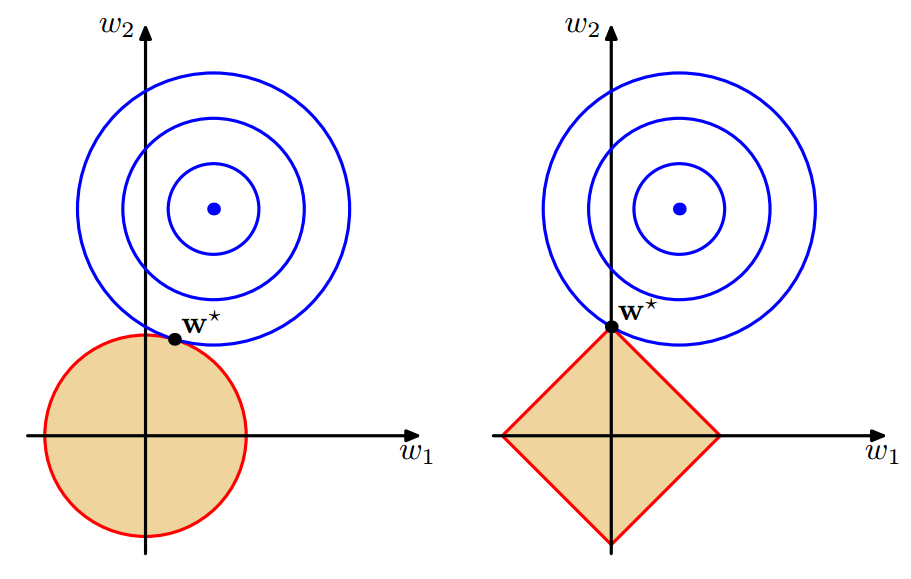
\includegraphics{PRML Part 1-1.eps} 
  \end{center}
  \caption{}
\end{figure}

Think about this figure in a Langrange-multipliers way.

\paragraph{Multiple outputs}\label{header-n81}

$\quad \quad$Of course we can decouple into multiple, independent regression
problems, however there is an approach using the same set of basis functions
so that y
\[ y (x, w) = W^T \phi (x) \]
and
\[ p (\mathrm{t} |x, W, \beta) = \mathcal{N} (\mathrm{t} |W^T \phi (x),
   \beta^{- 1} I) \]
which yields
\[ W_{ML} = \Phi^{\dagger} T \]
For the case of arbitrary covariance matrices, see MAL of multi-variate
Gaussian distribution.

\end{document}
